\chapter{Experimental Methods}
In this chapter I will describe the experiments I conducted for this thesis. The first section will deal cover the configuration and customization of the continuous wave (CW) Titanium Sapphire laser I used as an excitation source for conducting both PLE and $\mu$PL experiments. Section two will cover the design and construction of the in-cryostat optic mount for the $\mu$PL experiment as well as the optical configuration for data collection. Section three will illustrate the data collection procedure used in $\mu$PL experiments, as well as the function and implementation of LabView code I wrote for hardware control and data acquisition. In section four, I will lay out the optical design of our PLE experiments and in section five, I will discuss the experimental data collection process and signal optimization routines.

\section{The Light Source}
\indent The PLE and $\mu$PL experiments required a CW laser light source with a few properties: the laser must be a stable and fairly high-power light source with narrow line-width. For $\mu$PL, it was important that we have a fairly Gaussian and symmetric beam so we could obtain the desired spot-size and resolution at the sample. Additionally, conducting PLE scans required that we have the ability to computer control the laser wavelength over a fairly broad range of wavelengths, roughly a spectral region from $\lambda = 780$nm to $\lambda = 850$nm. The laser we chose for this task was a Schwartz Electro Optics Titan-CW Titanium Sapphire (Ti:Sapph) laser. Its specifications were fairly close to our needs, as its specified operating power is 500mW with a tunable range from roughly 700-820nm CITE Titan manual. 

\indent The laser cavity can be configured for either CW or pulsed operation. In CW operation a 532nm pump beam, 5W of power, enters the cavity through a series of steering mirrors. After entering, the pump passes through a lens to focus the pump on the Ti:Sapph crystal. After the gain medium, the remaining pump light passes through the end mirror and terminates at the back of the laser enclosure. The laser configuration is shown in figure 3.1.
\begin{figure}[h!]
\centering
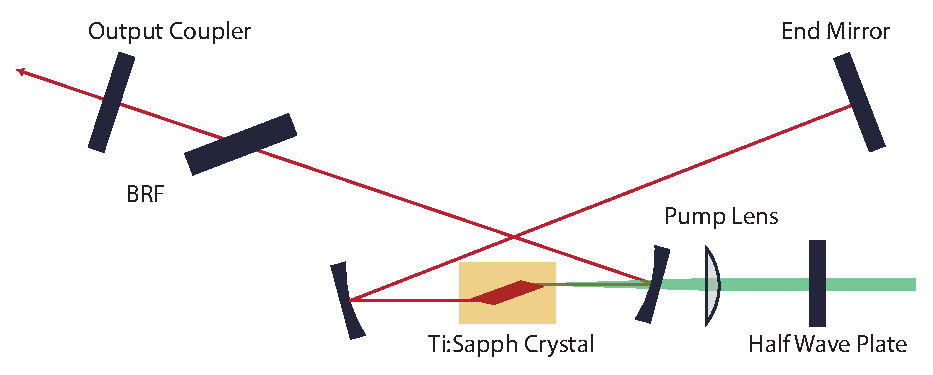
\includegraphics[width = .7\textwidth]{laser.eps}
\caption{ \doublespacing A depiction of the modified mount: the actuator arm fits into a sleeve attached by a pivot to the rotating filter mount. A spring attached to both the rotating mount and aluminum block holds the sleeve to the actuator and ensures smooth rotation in either direction.}
\label{lasercav}
\end{figure}

\indent Though the Ti:Sapph laser nearly met our specifications, it required two modifications to be operable in our experiments. First, we needed to add a computer controlled actuator to rotate the the birefringent tuner in order to allow for increased tenability and repeatability relative to a manually actuated micrometer. We modified the rotation mount for the birefringent filter (BRF) to accommodate a Newport TRB25 linear actuator. The linear actuator pushed a spring-loaded arm to rotate the BRF to a specified angle and select our desired wavelength. Figure 3.2 depicts the modified BRF mount with Newport actuator attached.
\begin{figure}[h!]
\centering
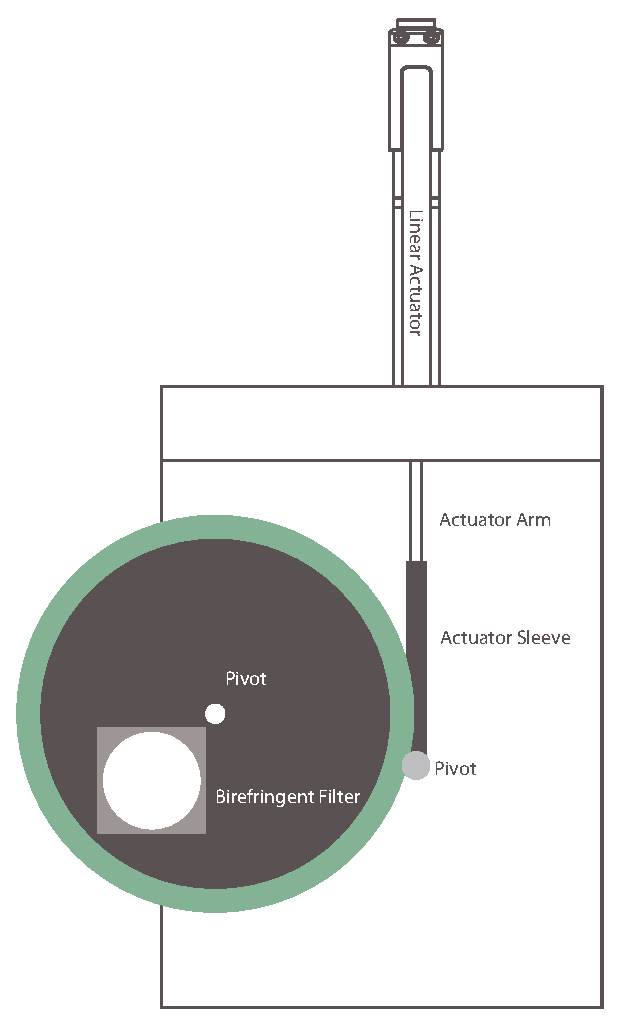
\includegraphics[width = .35\textwidth]{Actuator.eps}
\caption{ \doublespacing A depiction of the modified mount: the actuator arm fits into a sleeve attached by a pivot to the rotating filter mount. A spring attached to both the rotating mount and aluminum block holds the sleeve to the actuator and ensures smooth rotation in either direction.}
\label{brfmount}
\end{figure}

\section{Optical Components and Optical Path Configuration}

\subsection{Manufacturing the SIL}

\indent In order to obtain the resolution necessary to image disorder, the experiment employed a solid immersion lens (SIL) at the surface of the sample to increase the index of refraction at the imaging plane. I chose ZnSe as the SIL material, as its index of refraction at 780nm is n=2.4 CITE website. However, ZnSe SILs are not commercially available, so I resorted to manufacturing SILs from a stock ZnSe window. The window measured 2.54cm diameter by 1cm thickness, and our goal was to manufacture SILs of roughly 3mm in radius. To begin, we used a core drill, diameter 6.35mm, to cut out a cylindrical chunk of ZnSe. I then centered and glued the cylindrical stock material to a brass dowel, 2mm in radius. After the ZnSe was glued to the rod, the SIL shaping began. I put the brass dowel in a power drill used 200 grit sandpaper to shape the ZnSe cylinder roughly into a hemisphere.

\indent  When the SIL was in the roughly correct shape, we lapped and polished the hemispherical surface until the SIL was at the correct size. Additionally, since the experiment required optical quality surfaces, this was a careful and fairly lengthy process. I made the polishing lapps by machining a 2.54cm diameter copper rod to roughly 2cm in diameter with a 1.8cm wide by 1cm deep cavity. Then, I melted lead solder into the cavity, let it harden, and machined the face of the copper and solder until they were flush and mahcine-smooth. Then, I pressed a cleaned, 6.35mm dieameter ball bearing halfway into the solder. Figure 3.3 depicts what a finished lapp looked like before it was used to grind and polish the SIL. 

\begin{figure}[h!]
\centering

\includegraphics[width = .3\textwidth]{lapp.eps}
\caption{ \doublespacing A depiction of the lapp. The orange casing is copper while the grey lining is lead solder. The cavity left by the ball bearing was smooth enough to polish the relatively soft ZnSe hemispheres.}
\label{lapp}
\end{figure}



\indent After the lapp was made, we mounted the dowel with the SIL still attached to a glass lathe. As the lathe rotated, we placed the lapp with a mixture of glass polishing solution of various grit and mineral oil onto the SIL and held it in place with a sharpened wire. The wire and Lapp were both off center so the friction of the rotating SIL would randomly move the lapp so as to evenly polish the surface of the hemisphere. A depiction of this setup is in figure 3.4. (GRIT SIZE INFO). After the polishing process finished, the SIL was removed from the dowel and the flat surface was poilshed with a colloidal silicon mixture. When the SIL was finished, we had a hemispherical (to within 1\%) ZnSe SIL.

\begin{figure}[h!]
\centering

\includegraphics[width = .8\textwidth]{lathe.eps}
\caption{ \doublespacing A depiction of the polishing setup in the lathe. The off-center placement of the lapp and lapp pin allowed the lapp to rotate and move slightly to randomize the SIL polishing.}
\label{polish}
\end{figure}
\section{Cryostat Optics}